\section{Planteamiento del problema}
En la Escuela Profesional de Ciencia de la Computación de la Universidad Nacional de San Agustín se hace uso de una hoja de cálculo para listar la disponibilidad de libros de la biblioteca. Como se muestra en la figura \ref{fig:unsa-biblio1}, los datos pueden ser fácilmente afectados ya que podríamos alterar una fila o columna inadvertidamente.
\begin{figure}[H]
  \centering
  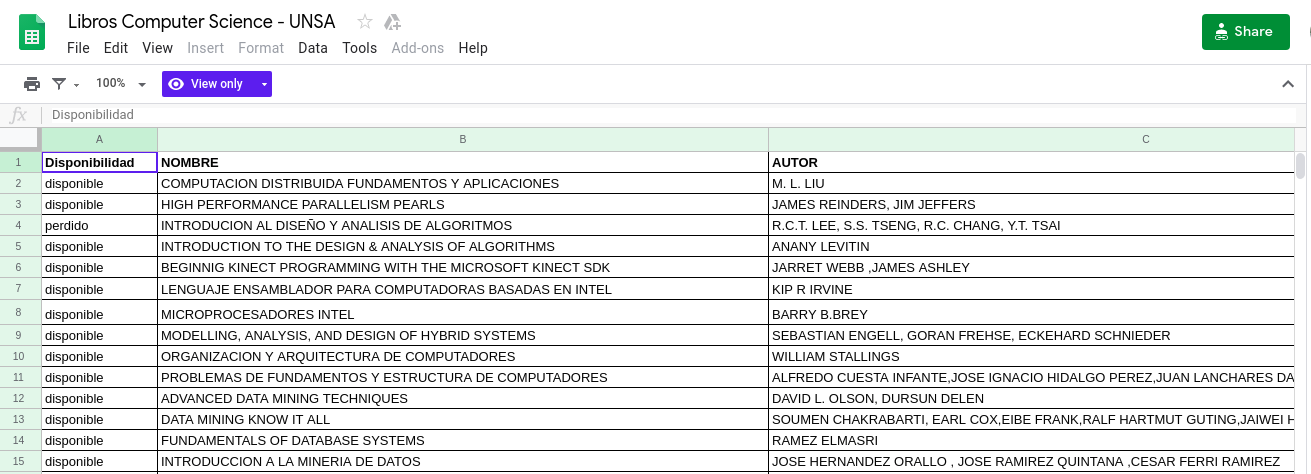
\includegraphics[width=0.9\textwidth]{UNSA-biblioteca_1}
  \caption{Uso de una hoja de cálculo para mostrar libros}
  \label{fig:unsa-biblio1}
\end{figure}

Además de que sería díficil mantener un registro de las personas a las cuales se les presto un libro, tal como se muestra en la figura \ref{fig:unsa-biblio2}.
\begin{figure}[H]
  \centering
  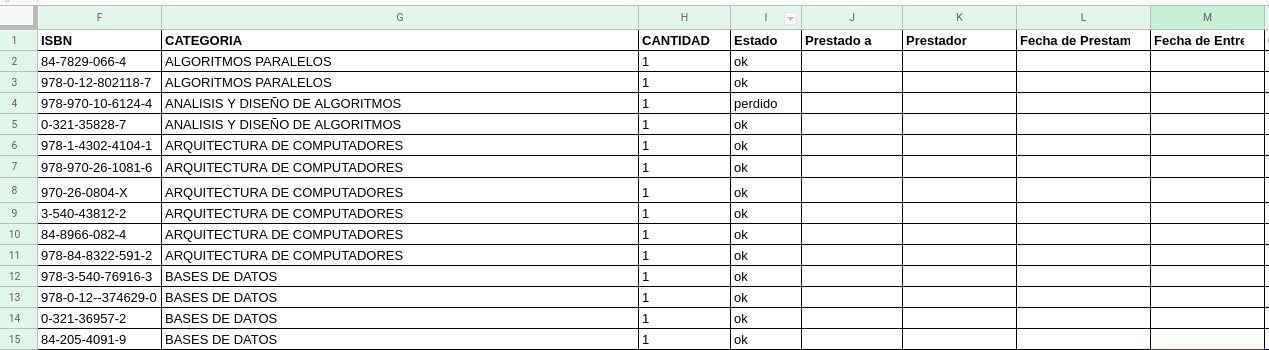
\includegraphics[width=0.9\textwidth]{UNSA-biblioteca_2}
  \caption{Uso de una hoja de cálculo para administrar libros}
  \label{fig:unsa-biblio2}
\end{figure}